\chapter{FIELD INTRODUCTION (Jakub Kinder)}
\label{chap:FieldIntroduction}

The main goal of this chapter is to present current information about PC building and its market.
It consists of descriptions of components and their compatibility, the assembly process as well as the most popular tools used to aid people both novice and experienced in the field.
However, it also explores currently available simulators, and how advanced and precise they are.
Another topic of this chapter is how VR as an environment is used and what advantages it has in the context of hardware assembly and visualization.

\section{PC building}
Nowadays, computers are built using modular components, which simplifies their construction and allows for immense flexibility regarding choice of components.
However, as mentioned in \autoref{chap:Introduction}, PC building still requires comprehensive knowledge not only about the process itself, but also the parts, their ports and physical dimensions.

\subsection{Components, ports and compatibility}
Every single component used in PC building possesses either a port, socket or connector with specific version or standard, which dictates compatibility with other components.
Furthermore, some parts have even stricter rules, requiring specific parametric matching to ensure proper function and physical fit within the enclosure.

\subsubsection{CPU}
Commonly known as the brain of a PC, the CPU is connected to a dedicated socket on the motherboard.
Compatibility is fundamentally spit across to manufacturers, Intel and AMD, which utilize incompatible connections standards.
Intel uses Land Grid Array (LGA), while AMD uses Pin Grid Array (PGA) or derived technology.
In addition, both types have their versions and sets of supported architectures, which means not every CPU will fit the same socket even if the type and version is matched.

Critical compatibility parameters:
\begin{itemize}
	\item Socket type: As mentioned above, For CPU to be compatible with a motherboard, the socket must match CPU's type, version and architecture.
	\item RAM controller limit: CPUs can support only specified amount of RAM, number of channels and RAM module's frequencies.
\end{itemize}

\subsubsection{RAM}
This component serves as system's primary volatile storage.
Its compatibility is perhaps the most nuanced of all parts used in PC building, as it is not only limited by CPU, but also RAM module's physical dimensions are a major factor in its compatibility with other components.
In addition, RAM uses Double Data Rate Synchronous Dynamic Random-Access Memory (DDR SDRAM or commonly referred to as DDR) technology, which uses Dual In-Line Memory Module (DIMM) slots.

Critical compatibility parameters:
\begin{itemize}
	\item Generation: Currently there are several generations of DDR available, most recent are DDR4 and DDR5. 
	Unfortunately, DDR technology is not compatible across its generations, so if port utilizes DDR4, RAM of no other generation can be installed in it, as is stated in Micron Technology's article \cite{noauthor_whats_2025}.
	\item RAM frequency: This aspect is the reason why RAM is considered one of the more nuanced components. 
	As mentioned earlier, CPU can support only specified values of this parameter, but the range of accepted frequencies is also limited by the motherboard, which also supports only specified values.
	In addition, all installed sticks of RAM must have the same value of this parameter, however, unlike CPU, they do not have the manufacturer constraint.
\end{itemize}

\subsubsection{GPU}
A specialized piece of hardware responsible for rendering graphics, which is more often than not, a critical component in most PCs.
It utilizes Peripheral Component Interconnect Express (PCIe) x16 interface for connection with the motherboard.
Unlike previously mentioned CPU sockets or RAM slots, PCIe is forwards and backwards compatible standard as is stated in Intel's article titled "What Are PCIe 4.0 and 5.0?" \cite{noauthor_what_nodate}.
This means that GPU with currently the newest PCIe version 5 can be connected to a version 4 slot and vice versa.
The only drawback with such connection is loss of performance, due to lower bandwidth on the side with lower version.

\subsubsection{Memory drive}
This component is usually either a Solid State Drive (SSD) or Hard Disk Drive (HDD), regardless of the type, its purpose is to store data long term.
The main differences between the two types are read/write speeds, in which SSDs are superior, and total amount of storage, which HDDs excel at.
Despite their differences, both types of memory drives utilize the same connection standard, Serial Advanced Technology Attachment (SATA).
Currently, there are three versions of this standard, SATA I, SATA II and SATA III, and just like PCIe, this standard is backwards compatible, with the drawback being drop of bandwidth to that of the lower standard. \cite{noauthor_what_2023}
Additionally, there is another type of memory drive called Non-Volatile Memory Express (NVMe), which instead of SATA, uses M.2, a PCIe x4 interface form factor.
These drives have even higher read/write speeds than regular SSDs, while offering similar amount of storage with the drawbacks being slightly shorter lifespan of the drive and the fact that not all motherboards have PCIe x4 slots.

\subsubsection{Motherboard}
This is the most crucial component in terms of compatibility, because every component mentioned above connects to it.
The motherboard determines, which CPUs, RAM modules, and memory drives can be installed.
Another important aspect for the motherboard is its form factor, the physical dimensions of the component.
The most common standard is Advanced Technology Extended (ATX), which states that motherboard should be 305 x 244 mm.
However, there are smaller standards like mini- Information Technology Extended (ITX) with dimensions of 170 x 170 mm.

Critical compatibility parameters:
\begin{itemize}
	\item CPU socket: As mentioned in CPU's compatibility, the connected CPU's connector must match the socket as well as CPU's architecture must be included in supported list of architectures of the motherboard.
	\item RAM: In this case compatibility is the most complicated as it was stated in RAM description. 
	Not only RAM modules must meet previously discussed requirements, but also they should be included in Qualified Vendor List (QVL) of the particular motherboard.
	\item Form factor: Motherboard's size, critically affects how other components are compatible with it on a more physical level, with ATX standard there might not be any issues, however, mini-ITX offers far less space which can prove problematic for components like RAM modules or GPUs.

\end{itemize}

\subsubsection{Power supply}
Power supply as the name suggests provides power to all the other components, which makes determining its compatibility straightforward.
It must deliver enough power to the computer, but while condition is simple it is one of the most important ones as not meeting it might result in damaging other components caused by improper function due to lack of power.

\subsection{The process of PC assembly}
Due to modular design of modern day computers, assembly in itself is straightforward, but still requires caution as some components require counterintuitive strength to be installed.
Most books and guides such as "Montaż komputera {PC}. {Ilustrowany} przewodnik" \cite{chabinski_montaz_2012} or Intel's guide on PC building \cite{noauthor_how_nodate} agree on general procedure of PC assembly, which is as follows:

\begin{enumerate}
	\item Before the actual assembly procedure, the case, that is to be used in the process must be prepared by removing its side and often front panels as well as screwing in separators on which the motherboard will be mounted.
	\item The first step of the building process is to install the CPU in the dedicated socket on the motherboard.
	It is done by opening the latch on the socket and very gently dropping CPU into it, followed by closing the opened latch.
	\item Optionally, after installing the CPU, NVMe drive can be installed if the motherboard possesses an M.2 slot.
	\item Next is to install RAM, first latches need to be unlocked on both sides of slots pointed out by motherboard's manual.
	Then, RAM modules are to be inserted into the slots, this operation requires counterintuitive amounts of force, thus prior to applying it, one must make sure that the modules are properly oriented, so as not to damage them or the slots.
	\item Afterward, the most common practice is to mount the power supply in previously prepared case, which is done according to case's manual.
	\item Subsequently, the partially assembled motherboard is to be installed in the case, be gentling placing it on the separators and screwing it in. 
	\item Next, the GPU must be installed, which is done by simply inserting it into the PCIe x16 slot on the motherboard and securing the component to the case using provided screws.
	\item The last components to be installed are the memory drives, if M.2 drives were already installed this step is optional.
	It is done be mounting the SSD or HDD drives in spots pointed out by the case manual, followed by connecting SATA cables to bot the drives and the ports on the motherboard.
	\item The final step of the assembly is to connect the power supply cables to the appropriate slots on other components, as well as connect smaller connectors leading from some components to the motherboard.
	These should be attached according to manuals of each component and the schematic included with the motherboard.
\end{enumerate}

\section{PC building market}
In recent years, PC building has become increasingly popular, majorly due to people's demand for customized and potentially more powerful devices.
For this reason, sales of PC parts have skyrocketed and so did the selection of purchasable components. 
According to most of the accessible reports on the PC parts market, like the report from PMarketResearch \cite{article} from the end of 2023, the gaming PC market alone was valued at approximately 18 billion USD and is expected to grow to around 200 billion USD by 2034.
Additionally, most recent and specific market reports are valued at 3,000 USD per copy.
Those facts show that the PC parts market is extremely volatile and rapidly expanding, so much so that just information on it is highly profitable.

\subsection{Existing PC building support tools}
The aforementioned rapid growth of the PC parts market is a direct result of heightened interest in PC building, which for years now has been supported by web applications that help choose compatible parts for a new machine.

\begin{enumerate}
    \item PCPartPicker \cite{PCPartPicker}
    
PCPartPicker is a popular tool for those interested in PC building. 
Its main features are simplified mechanic of choosing components and automatic compatibility guide which supports user in choosing proper components for their future machine. 
This solution also features categorized, sortable lists of components to limit the chance of providing too many choices at once.
The build page's main interface is presented on Figure \ref{fig:partpicker}.

\begin{figure}[!ht]
	\centering
	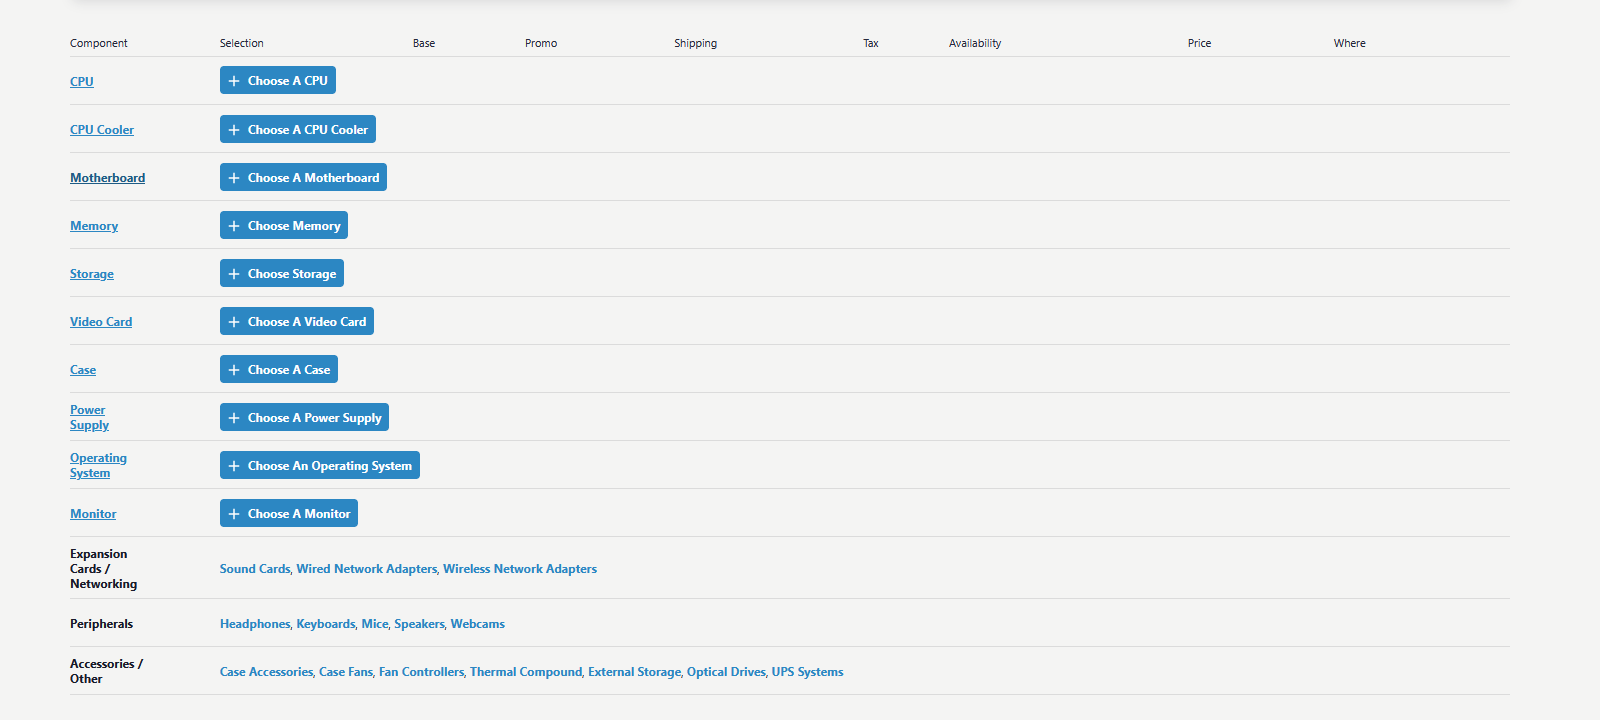
\includegraphics[width=0.6\textwidth]{Images/PCPartPicker.png}
	\caption{Screenshot of PCPartPicker.com build page}
	\label{fig:partpicker}
    \end{figure}

    \item BuildMyPC.net

This tool boasts itself on its simplicity, and while it accomplishes that it still overloads unexperienced users. 
It does it mainly through use of uncommon names of parts and including less used parts like network adapters, which usually are part of motherboards.
Those issues are shown on BuildMyPC.net's build page on Figures \ref{fig:buildmypc1} and \ref{fig:buildmypc2}
Aside from such a shortcoming, it remains as a popular aid tool for choosing a set of compatible PC parts.

\begin{figure}[h!]%
	\centering
	\subfigure[]{
		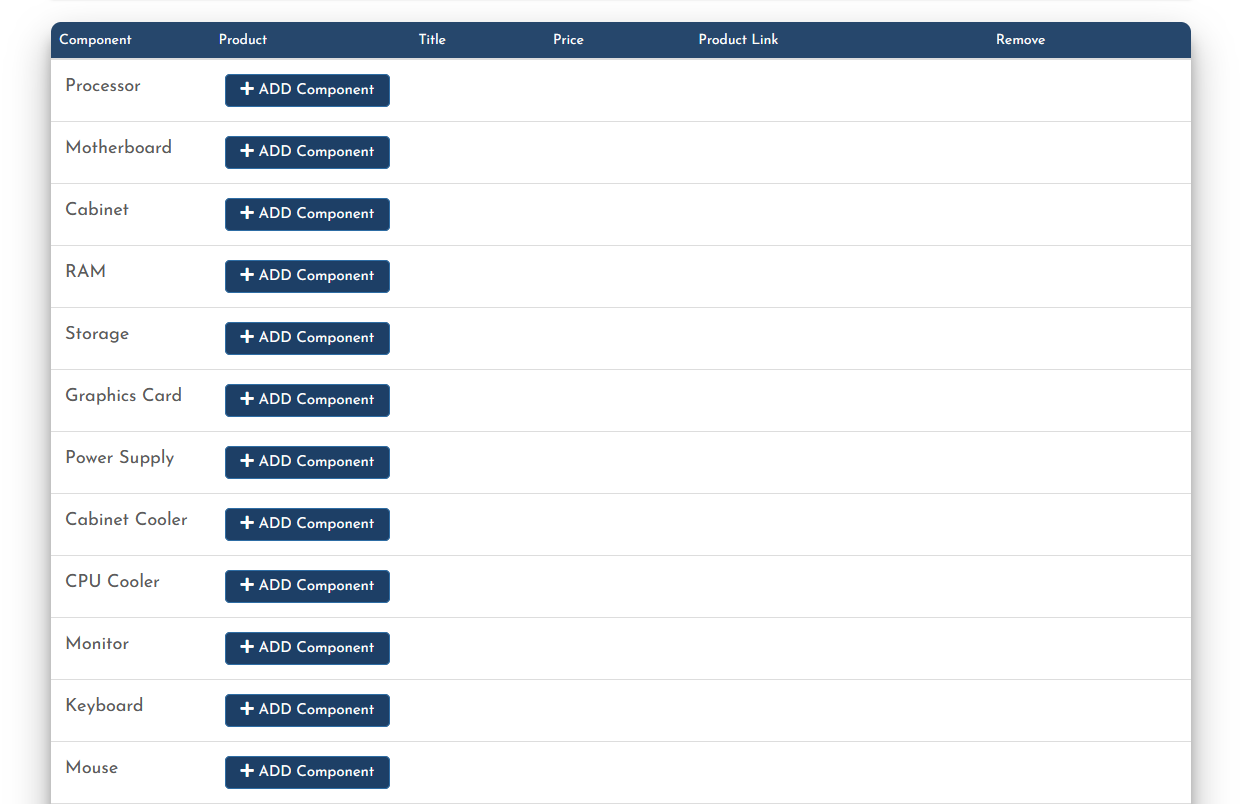
\includegraphics[width=0.48\textwidth]{Images/BuildMyPC.net1.png}
		\label{fig:buildmypc1}
	}%
	\hfil
	\subfigure[]{
		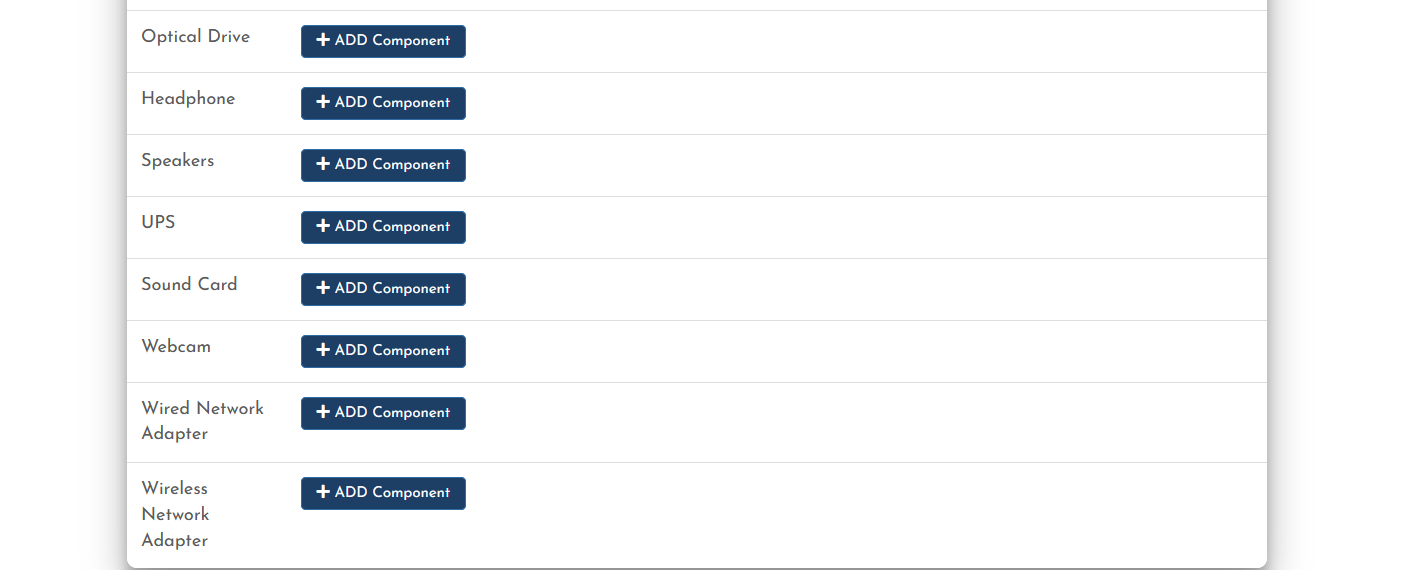
\includegraphics[width=0.48\textwidth]{Images/BuildMyPC.net2.png}
		\label{fig:buildmypc2}
	}
	\caption{Screenshots of BuildMyPC.net build page}
\end{figure}

    \item Logical Increments

    This item is a ranked list of PC parts which helps people choose  relatively up-to-date components to prolong longevity of newly built devices.
    The list consists of 16 ranks for each major PC part, like GPU, CPU, motherboard, SSD or HDD storage etc.
    Whats worth noting, is that each component is placed on the list based on many factors, mainly its based on components parameters but as it stands, the price also plays a major role in component's final placement. 
    Figure \ref{fig:logicalinstruments} presents small piece of mentioned list, and its notable feature is that each rank's sub-list can be further extended to view more parts. 

\begin{figure}[!ht]
	\centering
		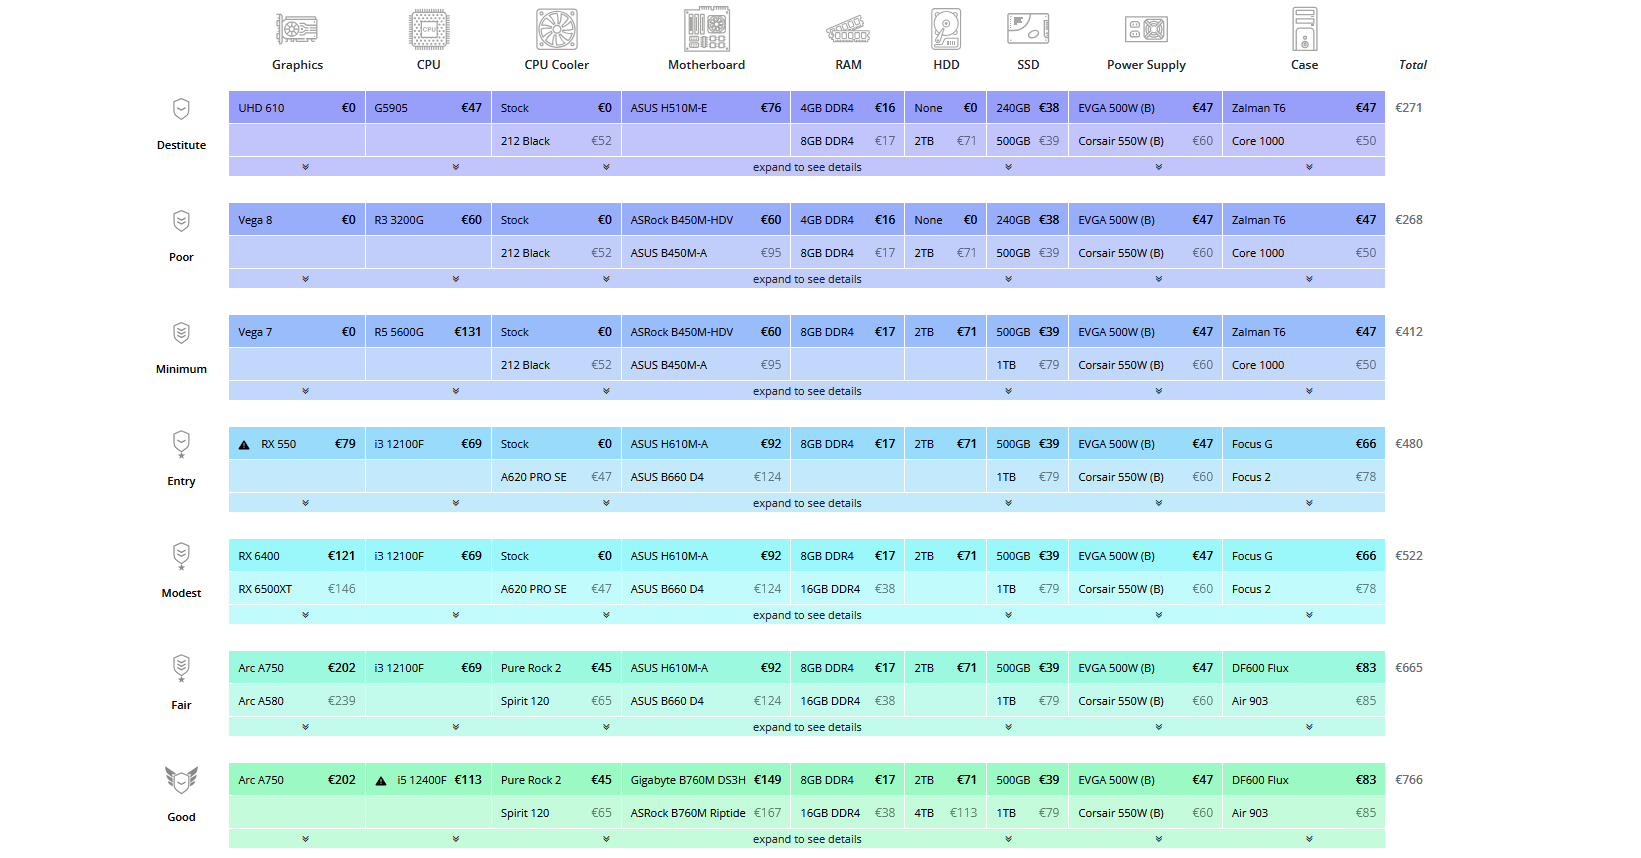
\includegraphics[width=0.85\textwidth]{Images/Logical_Instruments.png}
	\caption{Screenshot of a piece of Logical Instruments ranked list}
	\label{fig:logicalinstruments}
    \end{figure}
    
    \item PC Builder

This tool, while almost identical to PCPartPicker, features a more user friendly interface, ranging from visuals to phrasing of more specialized accessories, like thermal paste.
Its appearence can be observed on Figure \ref{fig:pcbuilder}.


\begin{figure}[!ht]
	\centering
		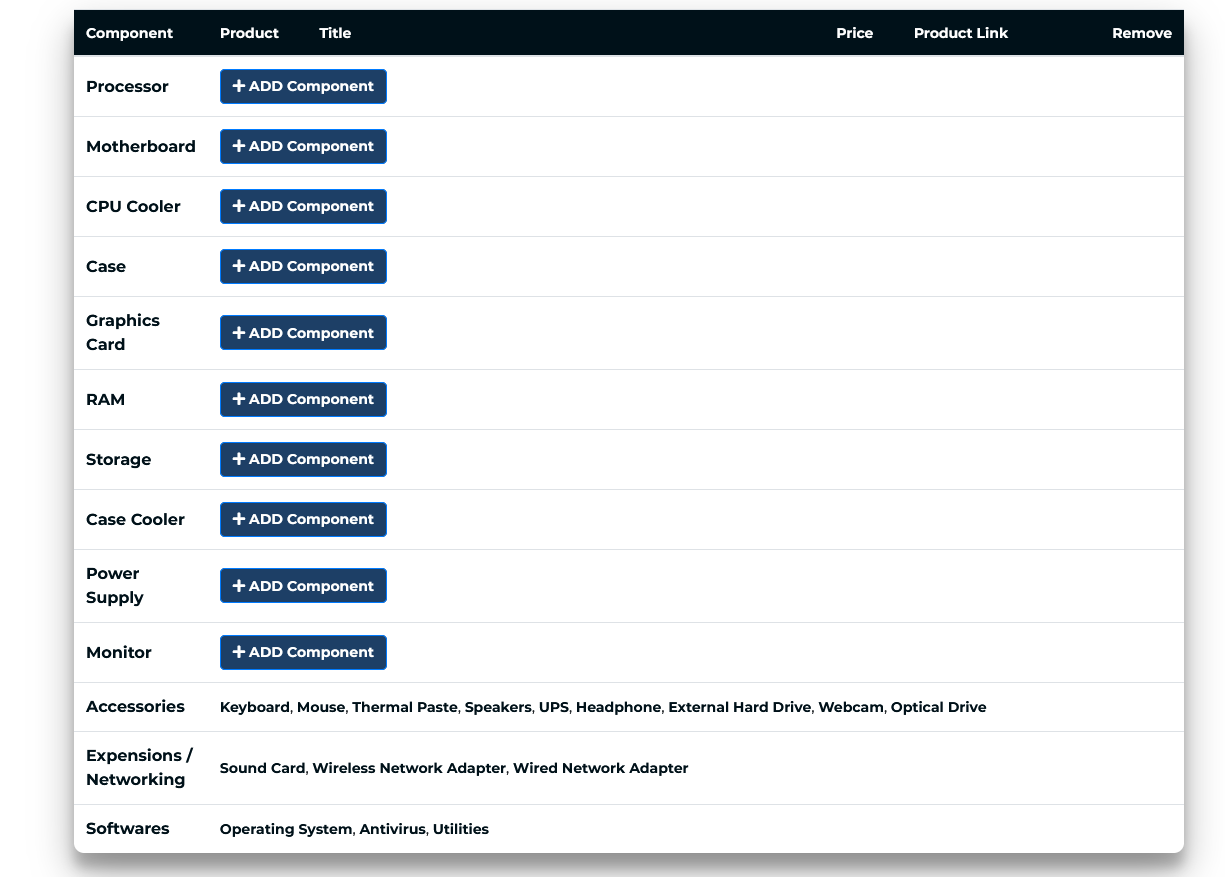
\includegraphics[width=0.7\textwidth]{Images/PCBuilder.png}
	\caption{Screenshot of a configuration component of pcbuilder.net website}
	\label{fig:pcbuilder}
    \end{figure}
    
    \item UserBenchmark

It is a comprehensive collection of over 350 million benchmarks of over 2 million unique components.
Additionally the website features a custom software for testing already built PC to check how well they will perform under current standards.
Other interesting features are, a compare module which allows uses to compare various components of given type and the other is voting system which allows users to rank specific components.
Aforementioned features can be observed on Figure \ref{fig:userbenchmark}.

\begin{figure}[!ht]
	\centering
		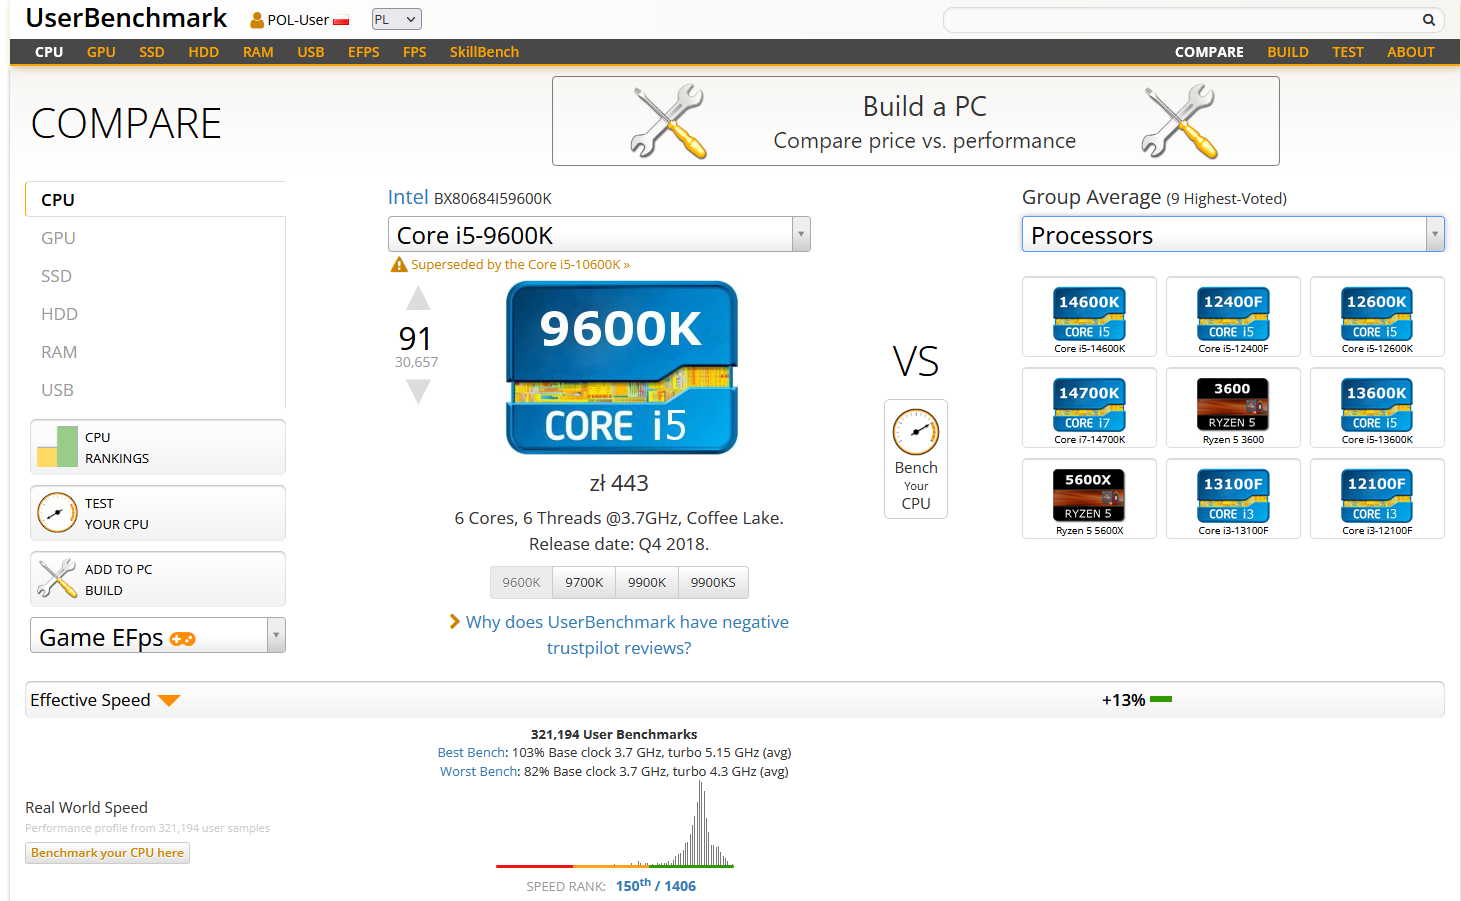
\includegraphics[width=0.7\textwidth]{Images/UserBenchmark.png}
	\caption{Screenshot of a UserBenchmark's CPU compare module}
	\label{fig:userbenchmark}
    \end{figure}
    
\end{enumerate}

\subsection{PC building simulators}
The market of PC building simulators is very limited when it comes to options.
In the desktop section alone, there are only 2 simulators, both from the same authors and in the same franchise.
Such circumstances make it hard to find an appropriate amount of material to base a new simulator on.
However, present options are comprehensive enough to satisfy the market, at least for simulators in a traditional 3D environment.

    \subsubsection{PC Building Simulator 1}
    
Released on 29th January 2019, PC Building Simulator 1 is a simulation game that pioneered PC building simulations in a 3D environment.
Before its release, the only tools used for aid in pc building were configuration apps, guides, and articles on the topic.
However, this game revolutionized the field by introducing actual 3D rendering of the components and featuring a simplified yet still realistic assembly process.

Apart from its origins, it is well known for its wide variety of rather realistically made PC part models.
Not only that, but this game features licensing from component manufacturers like Intel, AMD, NVIDIA, Corsair, and many others.
Figure \ref{fig:pcbspartners} presents a little over half of the manufacturers that the game has licenses from.
This allows for the parts to have real-world specifications, which provide extra information for players. 

\begin{figure}[!ht]
	\centering
		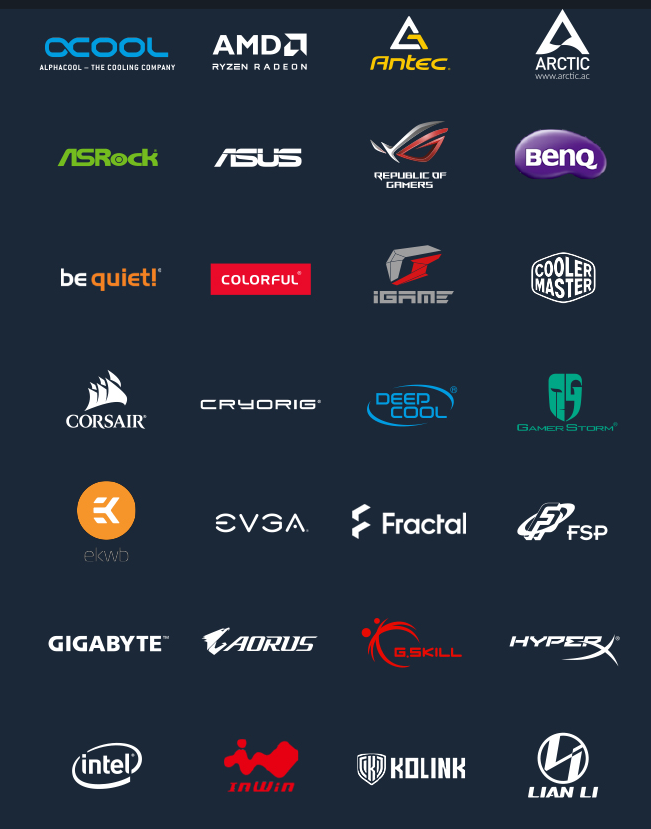
\includegraphics[width=0.4\textwidth]{Images/PCBuildingLicensing.png}
	\caption{Screenshot of a partial list of hardware partners from Steam page of PC Building Simulator.}
	\label{fig:pcbspartners}
    \end{figure}

The game emphasizes a rather realistic process of assembling computers, by not only implementing the installation of separate modules, but also including the process of cable management or creation of custom water cooling solutions.
Those features alone make it an incredibly valuable tool for learning how to build PCs, but the implemented mechanics don't stop there.
The application possesses robust visualization of devices' operation, including RGB lighting.
Also, it has a selection of downloadable content (DLC) which further expands available mechanics by adding the possibility of overclocking of the built PC.
Not only that, the game features a campaign / story mode, which greatly enhances its educational value.
The main advantages of this particular feature are tutorials and early guides for new players, that greatly advance their knowledge and theoretical skills in building a PC.
As for more advanced and knowledgeable about PC assembly, the game offers the ability to enter a virtual BIOS of in-game computers, allowing for finer tuning of settings.

\begin{figure}[h!]%
	\centering
	\subfigure[]{
		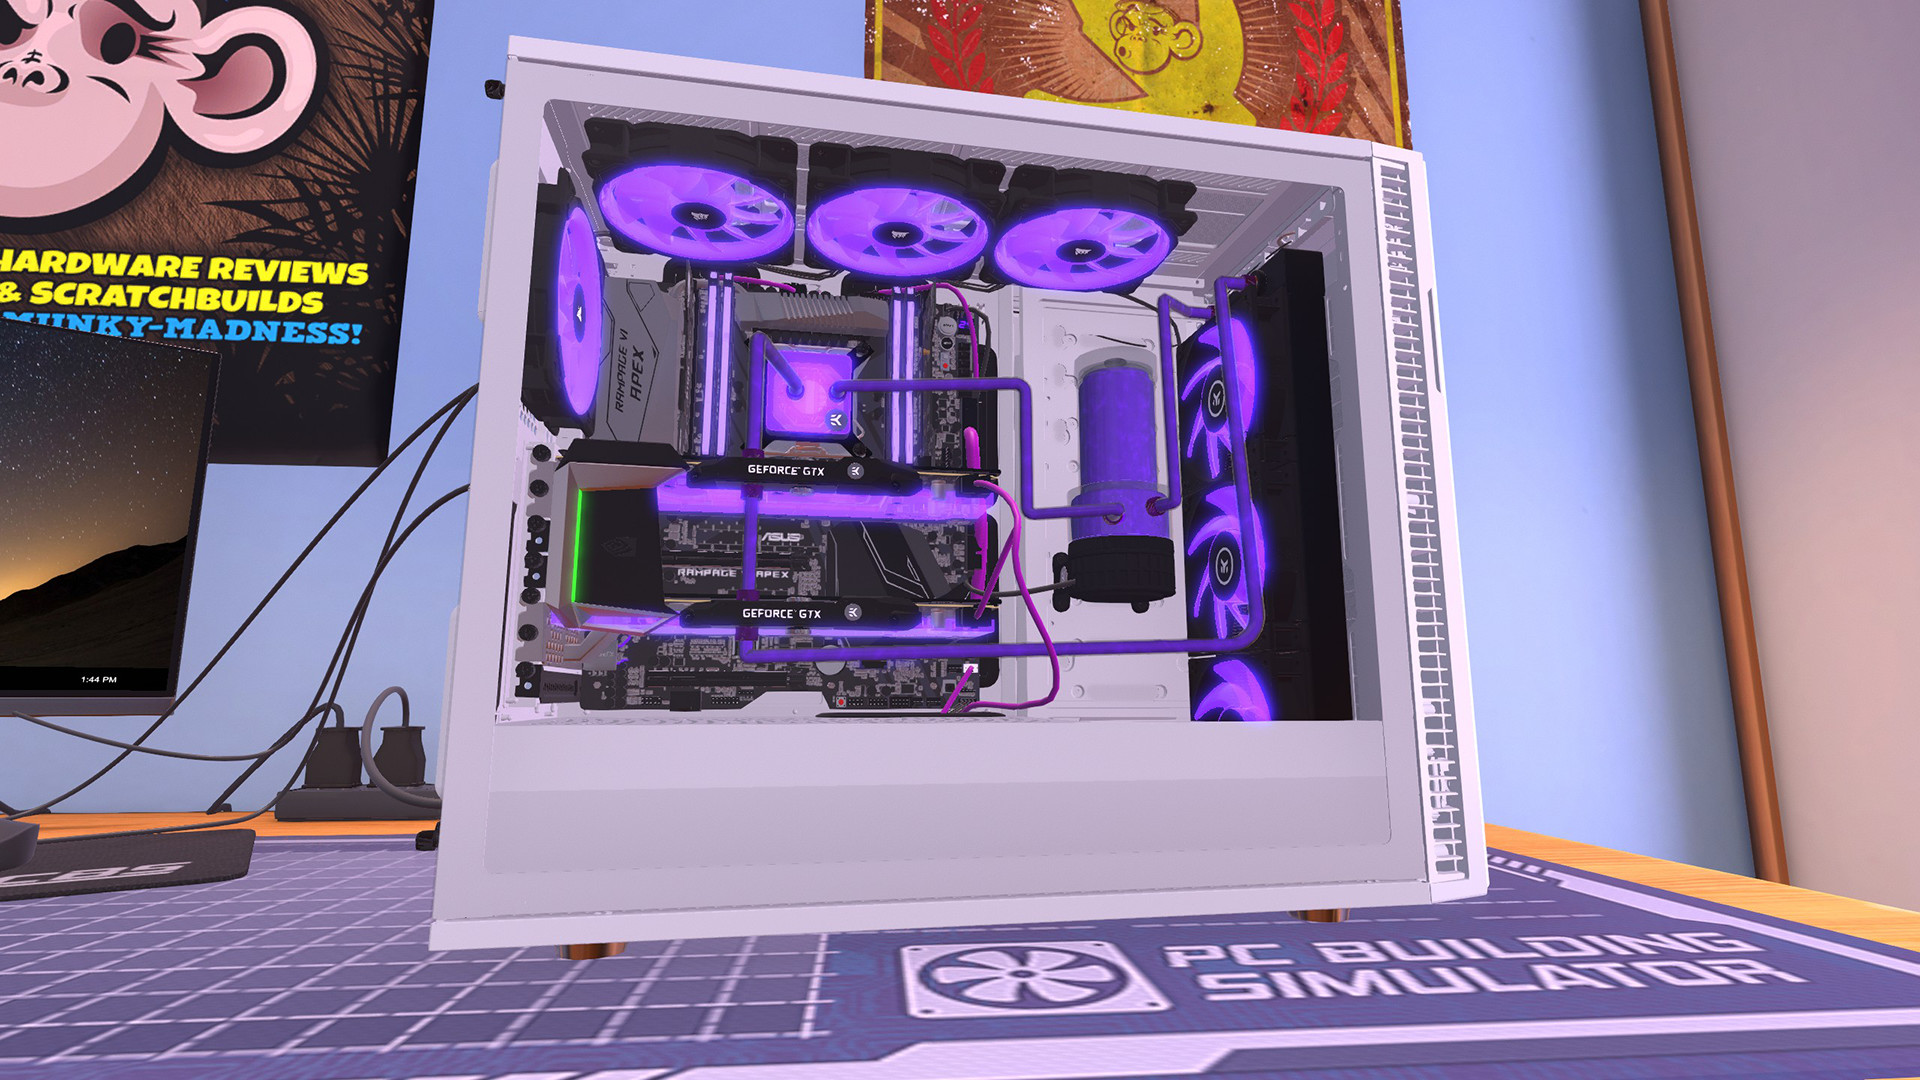
\includegraphics[width=0.45\textwidth]{Images/PCbuidlignSimulator1(2).jpg}
		\label{fig:pcbsbuild1}
	}%
	\hfil
	\subfigure[]{
		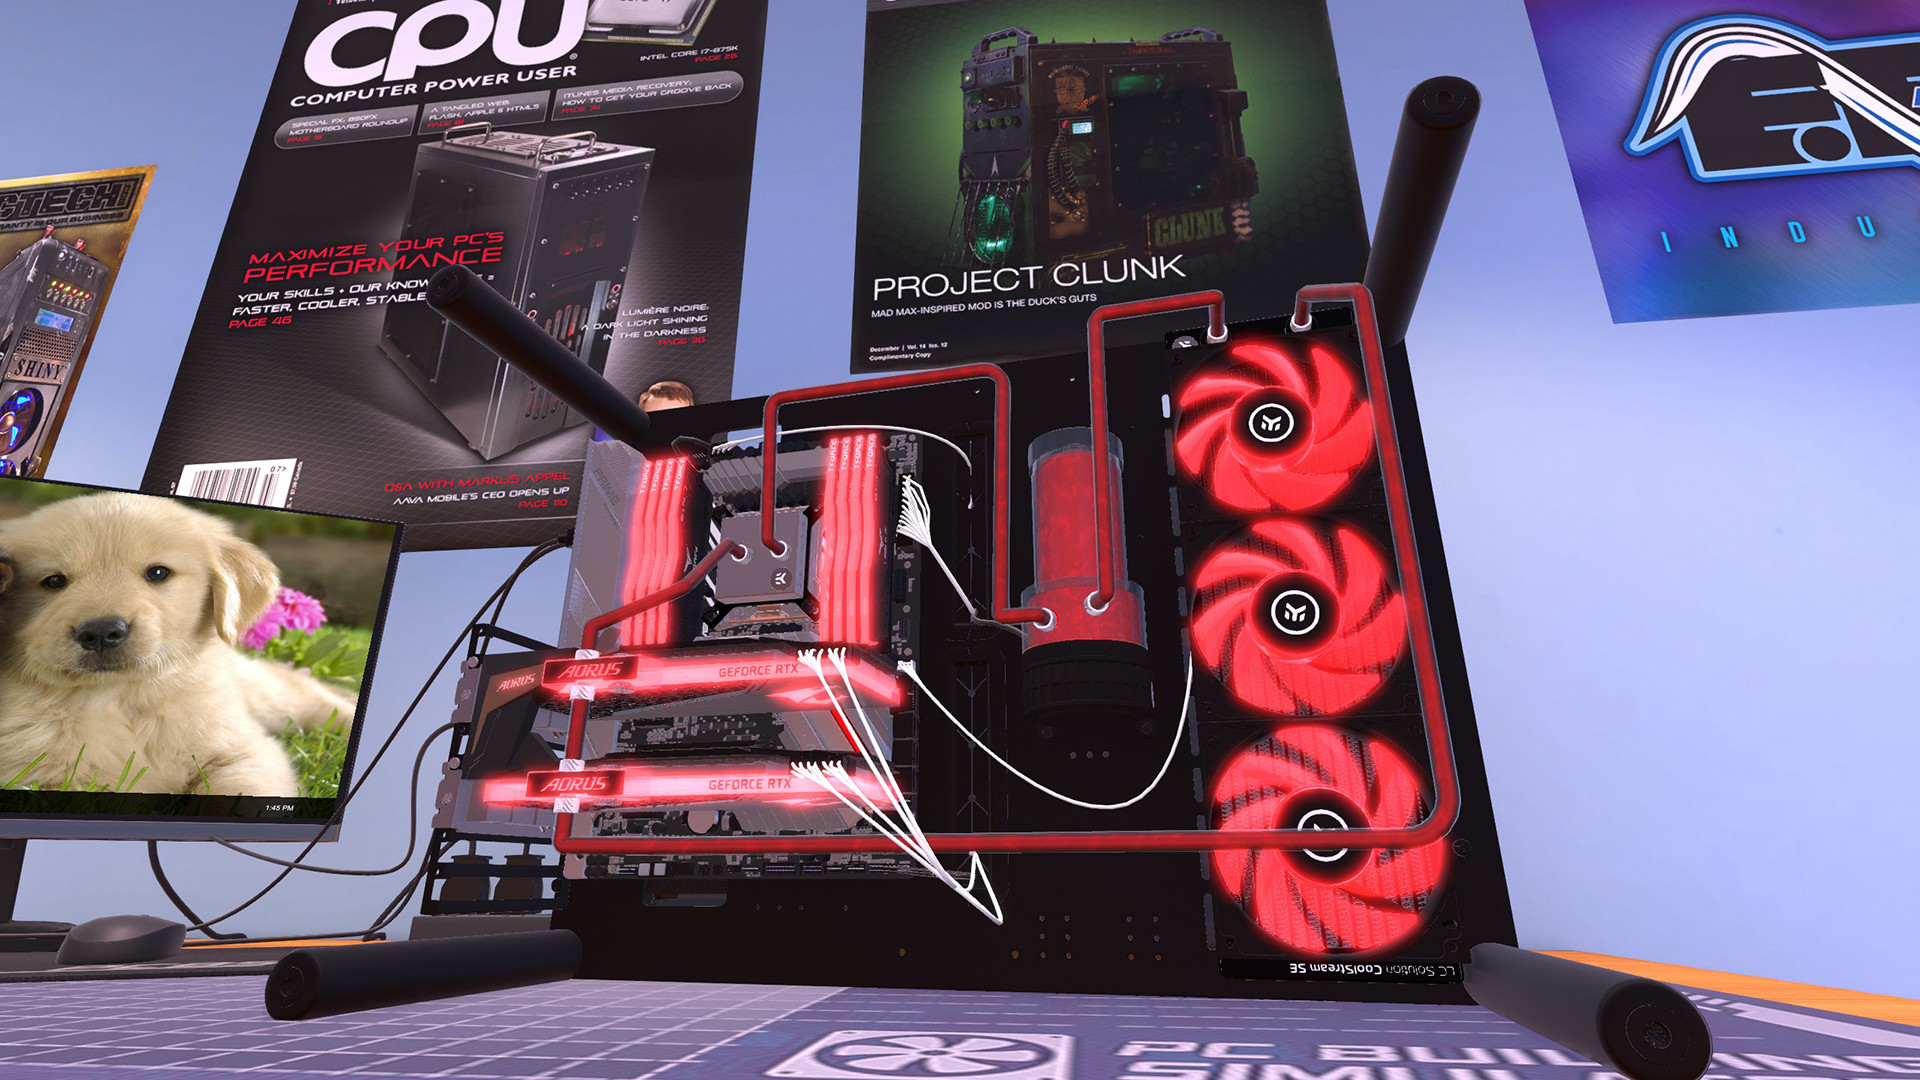
\includegraphics[width=0.45\textwidth]{Images/PCbuidlignSimulator1.jpg}
		\label{fig:pcbsbuild2}
	}
	\caption{Screenshots of a finished PCs made in PC Building Simulator from its Steam page}
\end{figure}

Figures \ref{fig:pcbsbuild1} and \ref{fig:pcbsbuild2} present possible PCs that can be built both in the game and in the real world, by utilizing mechanics and features described earlier.
Those possibilities are further expanded through the game's use of the Steam workshop feature, allowing players to make their own free DLCs.
This aspect of the game creates essentially endless options for assembling PCs that are realistic and feasible in the real world.

While PC Building Simulator is an incredibly comprehensive tool for gaining knowledge about PC building, it retains a rather low player count of an average of under 1000 unique players a month according to SteamDB.
Despite that, the game remains a popular and well-liked solution, as estimates of owned copies range from 1 to 4 million of both legally and illegally acquired copies.
Also, important factor in judging its usefulness is the reviews of its players on Steam.
Currently, there are slightly over 41 thousand reviews and 93\% of them are positive.

    \subsubsection{PC Building Simulator 2}

It is the second installment of the PC Building Simulator franchise, released on 12th October 2022.
It took the place of the best PC building simulator from its predecessor by implementing far more features and much better, more realistic graphics.
Also, its selection of components was vastly extended.

Just like the original PC Building Simulator, it has official partnerships with PC part manufacturers. However, this installment introduced many more than before, allowing for more niche parts to be included in an already large selection.
Also, unlike its predecessor, this game introduced partnerships with accessory producers like Thermal Grizzly, allowing for the players to get familiar with a wide selection of various PC building tools and products other than components like thermal pastes, pads, or even GPU stands.
Nonetheless, the biggest non-functional improvements upon the original are overhauled, realistic graphics; this is best showcased in Figure \ref{fig:pcbs2build}.

\begin{figure}[!ht]
	\centering
		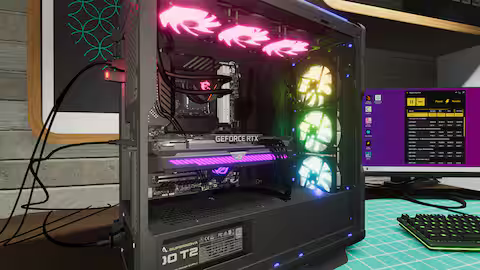
\includegraphics[width=0.65\textwidth]{Images/PCBuildingSim2.png}
	\caption{Screenshot of a finished PC made in PC Building Simulator 2 from Epic Games Store}
	\label{fig:pcbs2build}
    \end{figure}

The game also improved already revolutionary mechanics from the previous title by enhancing physics and models of all components.
This resulted in much better realism, but it also added many steps that were omitted in PC Building Simulator 1.
Some of the steps are:


\begin{itemize}
    \item Locking/unlocking CPU socket
    \item Application of thermal paste
    \item Installing I/O shields
\end{itemize}

While those steps tend to be mundane, they are crucial in building a functional PC and they require more precision than anyone expects.
Given that, PC Building Simulator 2 handles those and even more steps with a lot of care and realism.

Another new feature is the possibility to take apart some components like the GPU to further customize the PC by adding a less used water cooling block.
Also, it showcases how the GPU chipset actually looks like, giving players a far better understanding of what each component is.
Figure \ref{fig:pcbs2gpushipset} shows the taken apart GPU chipset being cleaned in-game, which is another new and interesting mechanic of this game.

\begin{figure}[!ht]
	\centering
		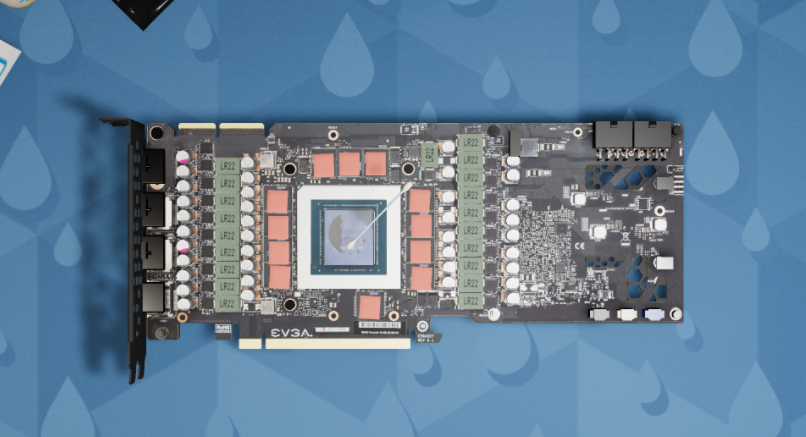
\includegraphics[width=0.7\textwidth]{Images/GPUChipsetPCBS2.png}
	\caption{Screenshot of a GPU chipset in PC Building Simulator 2 from Epic Games Store}
	\label{fig:pcbs2gpushipset}
    \end{figure}
    
Similarly to its predecessor, the game offers many tools to further customize virtual PCs.
Those tools consist of an expanded BIOS and even a fan curve control application; the latter is presented in figure \ref{fig:pcbs2fancurve}. 
Also, in this installment, the authors included benchmarks that simulate actual testing of assembled computers.

\begin{figure}[!ht]
	\centering
		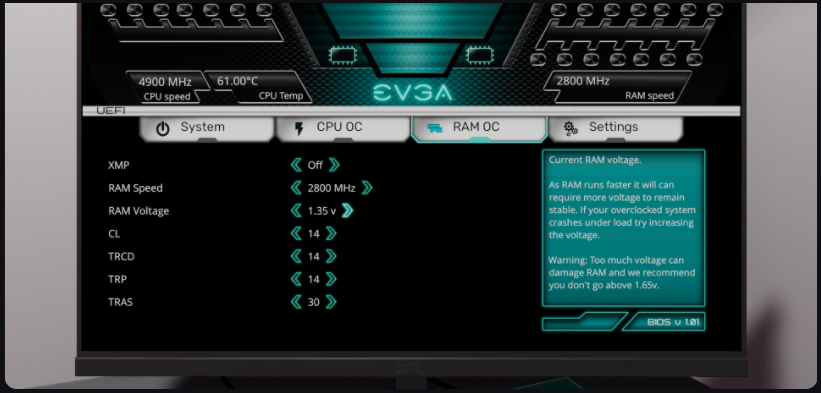
\includegraphics[width=0.7\textwidth]{Images/PCBS2FanCurveApp.png}
	\caption{Screenshot of fan curve application in PC Building Simulator 2 from Epic Games Store}
	\label{fig:pcbs2fancurve}
    \end{figure}

The aforementioned features already place it leagues above its predecessor and make it far better educational material on PC building.
However, the game has far more features that make it stand out.
With better graphics and physics, it reached a whole new level of visualization of the operation, and new customizing mechanics add new, less popular avenues to explore for those already advanced in PC assembly.

Unfortunately, this installment of the franchise didn't gather as much recognition as its predecessor.
Mainly, it is due to the choice of platform by the authors to sell their product, Epic Games Store.
It's worth mentioning that at the time of the game's release, Epic Games Store was widely hated for its exclusive program, which meant that any games under such contract could only be sold by Epic Games.
This combination led to an almost automatic decrease in the popularity of any games sold solely on this platform, and as we have discussed, PC Building Simulator 2 was one of the games that suffered from it.

\section{VR in hardware assembly and simulations}
\label{sec:VRGamesAndSimulations}

VR has seen increased use across a broad spectrum of industries, from gaming and education to medicine and engineering. In the context of hardware simulation, VR offers an immersive environment where users can interact with complex components and systems more intuitively. This makes it an increasingly promising tool for simulating physical tasks like PC building, especially for educational or training purposes.

\subsection{Advantages of using VR in hardware simulations}

Unlike traditional, more advanced simulations that use a regular 3D environment, simulations in VR offer much greater interactivity and immersion with users' surroundings.
Also, it allows for a simpler implementation solution as natural, even instinctive movements don't have to be coded, but only tracked.
This expands possible fields that can be simulated as  well as enhances angles from which working hardware can be observed, which adds another layer of precision.
In other words, using VR in hardware simulations provides the following benefits:

\begin{itemize}
    \item Immersive learning environment
    \item Safe space to experiment with hardware
    \item Real-time feedback on user interactions
    \item Fewer constraints on location or scene construction
\end{itemize}

\subsection{Existing VR hardware simulators}

As stated before, VR is an excellent environment for more advanced simulations.
And many game studios, university students, and researchers have taken that opportunity to fill the void.
Currently, there are countless VR simulators of many different kinds.
However, there aren't any about PC building; the closest we can find are those about assembling machines or robots.
That means that even though there are more simulators than one can count, VR still offers avenues to be explored.

\subsubsection{Virtual milling machine simulator}

This is an application made for Cave Automatic Virtual Environment (CAVE), focusing on the visualization of the operation of a specialized milling machine.
It was made in a specialized laboratory of Gdansk University of Technology by its students in 2020.

What makes this simulator stand out is the level of detail at which each component of the machine is simulated.
Each moving component is animated and in a CAVE environment, just like in VR, one can view the machine from different angles and notice things that simply are not possible in a traditional 3D setting on a monitor.
Such an approach allows for much better visualization of complex machines and opens new safe ways of understanding them.

Another interesting feature is the specialized graphical user interface (GUI), which is not made from a template like most do these days.
Rather, it uses field-specific icons and adds hints like names of parts the user points towards, which allows for a far smoother interaction with the simulated environment and understanding of how the simulated machine operates.

\subsubsection{Virtual Industrial Robot Assembly Simulator}

This is another application made for CAVE, however this one focuses on assembling an industrial robot from given parts.
It was made in a specialized laboratory of Gdansk University of Technology by HHN in 2019.

This application was developed as a trainer for building robots in a timely manner by following visual hints.
What makes this application interesting is that parts that the user is supposed to use to assemble his robot are placed on shelves around, which gives him a slight sense of challenge to match the visual hint to the part he/she has to use next.

The building mechanic is rather simple, the user has to grab the right part and drop it in close proximity to the visual hint.
The biggest challenge is to find the exact part, as all parts are placed on shelves around the player, and some of them are very similar to each other.
However, the scene makes it easier to quickly navigate between shelves and locate appropriate parts in a timely manner.
Nonetheless, the simulator shines with its intuitive controls and simple mechanics.

This simulator is a prime example of what VR hardware building simulations are like.
Most of them feature a simple grab and drop model, which at the same time is simple to implement and intuitive.
However, this particular application implemented a part recognition function, so that the user cannot place a part in the wrong order or place.

%\section{Interest in PC building}
%\label{sec:InterestInPCBuilding}
